\documentclass[document.tex]{subfiles}
\begin{document}
\section*{Exercise 3:}

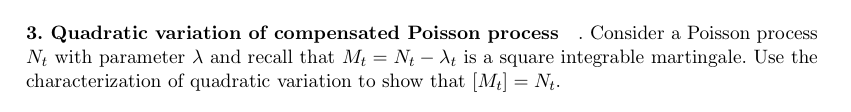
\includegraphics[width=\textwidth]{ex3.png}

Consider $M$ as an Ito integral $M=\int_0^t \theta_s dW_s$.
Then we have
\begin{align*}
	\qVar{M} &= \qcVar{M}{M} \\
	&=  \qcVar{\int_0^t \theta_s dW_s}{\int_0^t \theta_s dW_s} \\
	&= \int_0^t \theta_s^2 d \qcVar{W}{W}_s \\
	&= \int_0^t \theta_s^2 ds
\end{align*}
Therefore
\begin{align*}
	exp(M-\frac{1}{2}\qVar{M}) = exp(\int_0^t \theta_s dW_s-\frac{1}{2}\int_0^t \theta_s^2 ds
) 
\end{align*}
Now we can apply Girsanov Thereom and know $exp(M-\frac{1}{2}\qVar{M})$ is a local martingale.   
\end{document}
